\documentclass{beamer}
\usepackage{graphicx}
\usepackage{listings} % Syntax highlighing
\usepackage{fancyvrb} % Inline verbatim
\usepackage{hyperref} % Hyperlinks
\hypersetup{pdfpagemode=FullScreen}
\usepackage{tikz}
\def\checkmark{\tikz\fill[scale=0.4](0,.35) -- (.25,0) -- (1,.7) -- (.25,.15) -- cycle;}

\usetheme{Boadilla}
\title{Analysis \& Curation}
\author{UMBC Malware Data Science}
\date{Week 2: 4 February 2020}

\begin{document}

\begin{frame}
    Recap: Last week we discussed malware, and methods to study an unknown binary. The lab introduced you to Ghidra.
\end{frame}

\section{Static Analysis}
\begin{frame}{Static Analysis}
    Static features can come from a variety of sources:
    \begin{itemize}
        \item The strings command
        \item Disassembly
        \item Identifying system calls
        \item Finding embedded content
        \item $N$-grams
        \item Python and the \textit{pefile} module
        \begin{itemize}
            \item \href{https://www.usenix.org/legacy/events/leet09/tech/full_papers/wicherski/wicherski_html/index.html}{pehash}
            \item \href{https://www.fireeye.com/blog/threat-research/2014/01/tracking-malware-import-hashing.html}{imphash}
        \end{itemize}
        \item Similarity hashes
        \begin{itemize}
            \item \href{https://ssdeep-project.github.io/ssdeep/index.html}{ssdeep}
            \item \href{http://roussev.net/sdhash/sdhash.html}{sdhash}
            \item \href{https://github.com/EdwardRaff/LZJD}{LZJD}
        \end{itemize}
    \end{itemize}
\end{frame}

\begin{frame}{File Type Identification}
    But first, check the file type!
    \begin{itemize}
        \item Magic number
        \item \textit{file} command (libmagic)
    \end{itemize}
    \\ ~~ \\
    Why? Because malware authors lie.
    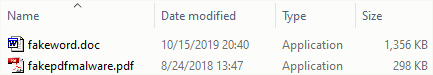
\includegraphics[width=0.65\columnwidth]{Images/fake_apps.png}
\end{frame}

\begin{frame}{Magic Numbers}
    \begin{table}
    \begin{tabular}{l | c | c | c | c }
    File Type & Bytes & Decoded & File Extension \\
    \hline
    ELF & 0x7f454c46 & .ELF & no extension, .so \\
    PDF & 0x25504446 & \%PDF & .pdf \\ 
    PE32 & 0x4d5a & MZ & .exe, .dll, .sys, .scr, .ocx, .cpl \\
    \end{tabular}
    \end{table}
    \\ ~~ \\
    This is easy to check. Simple Python3 one-liner: \\ \texttt{isPE32 = lambda x: open(x, "rb").read(2) == b"MZ"} \\
    \texttt{>>> isPE32("/path/to/app.exe")} \\
    \texttt{True}
\end{frame}

\begin{frame}{libmagic}
    \begin{itemize}
        \item Run as: \texttt{file /path/to/file.ext}
        \item Example results:
            \begin{itemize}
                \item \texttt{fakepdfmalware.exe: PE32 executable (GUI) Intel 80386, for MS Windows}
                \item \texttt{somemalware.exe: PE32 executable (GUI) Intel 80386, for MS Windows, UPX compressed}
                \item \texttt{file.pdf: PDF document, version 1.5}
                \item \texttt{macos-binary: Mach-O 64-bit x86\_64 executable, flags:<NOUNDEFS|DYLDLINK|TWOLEVEL|PIE>}
                \item \texttt{linux-binary: ELF 64-bit LSB shared object, x86-64, version 1 (SYSV), dynamically linked, interpreter /lib64/l, for GNU/Linux 3.2.0, BuildID[sha1]=fb7619d02b764941472818341f4c46be0de02502, stripped}
            \end{itemize}
    \end{itemize}
\end{frame}

\begin{frame}[fragile]{Strings}
    The strings command produces usually unhelpful results
    \begin{columns}
    \column{0.5\textwidth}
        \small
        \begin{verbatim}
'*  KJJJ;t
mojj
 99MJJBy
9#KMJJ\
  =LMOO`
*1=R\QQc
*<=UUQ\h
*@@VU```g
2@CVVg`m
'2FCaccm
3F[Yam
[i(2
GtS2rd
7tS:rd
k&*cd
7ec*
*	t!
        \end{verbatim}
    \column{0.5\textwidth}
    \small
        \begin{verbatim}
eh_personality.cc
_signal
_malloc
_fclose
_strcpy
_write
_strlen
_read
_memmoveP
_rndname
__Z11GetUserPathv
__Z9FileExistPKc
__Z4OpenPKc
_HeaderDir
.text$_ZStorSt13_Ios_OpenmodeS_
__Z12CreateHeaderv
        \end{verbatim}
    \end{columns}
\end{frame}

\begin{frame}[fragile]{Strings}
    Sometimes, there's useful information
    \small
        \begin{verbatim}
eh_personality.cc <--- Embedded source code?
_signal <--- Catches OS signals
_malloc
_fclose <--- Close a file
_strcpy
_write  <--- Writing to a file
_strlen
_read  <--- Reading from a file
_memmoveP
_rndname
__Z11GetUserPathv <--- Get user home directory
__Z9FileExistPKc <--- Test file existence
__Z4OpenPKc
_HeaderDir <--- Directory for header files?
.text$_ZStorSt13_Ios_OpenmodeS_ <--- Opening a file
__Z12CreateHeaderv <--- Create a header file?
        \end{verbatim}
\end{frame}

\begin{frame}[fragile]{Disassembly}
\lstset{language=assembly,
                basicstyle=\tiny,
                keywordstyle=\color{blue}\ttfamily,
                stringstyle=\color{red}\ttfamily,
                commentstyle=\color{green}\ttfamily,
                morecomment=[l][\color{magenta}]{\#}
}
\begin{lstlisting}
             undefined __stdcall entry(void)
             undefined         AL:1           <RETURN>
             undefined2        Stack[-0x18]:2 local_18    XREF[1]:   00401316(R)  
             undefined4        Stack[-0x1c]:4 local_1c    XREF[2]:   004012ec(RW), 
                                                                      0040130e(R)  
             undefined1        Stack[-0x48]:1 local_48    XREF[1]:   004012f0(*)  
                             entry                XREF[2]:   Entry Point(*), 00400100(*)  
        004012af 55              PUSH       EBP
        004012b0 8b ec           MOV        EBP,ESP
        004012b2 83 ec 44        SUB        ESP,0x44
        004012b5 56              PUSH       ESI
        004012b6 ff 15 18        CALL       dword ptr [->KERNEL32.DLL::GetCommandLineA]
                 20 40 00
        004012bc 8b f0           MOV        ESI,EAX
        004012be 8a 06           MOV        AL,byte ptr [ESI]
        004012c0 3c 22           CMP        AL,0x22
        004012c2 75 14           JNZ        LAB_004012d8
                             LAB_004012c4                                    XREF[1]:     004012ce(j)  
        004012c4 8a 46 01        MOV        AL,byte ptr [ESI + 0x1]
        004012c7 46              INC        ESI
        004012c8 84 c0           TEST       AL,AL
        004012ca 74 04           JZ         LAB_004012d0
        004012cc 3c 22           CMP        AL,0x22
        004012ce 75 f4           JNZ        LAB_004012c4
                             LAB_004012d0                                    XREF[1]:     004012ca(j)  
        004012d0 80 3e 22        CMP        byte ptr [ESI],0x22
        004012d3 75 0d           JNZ        LAB_004012e2
\end{lstlisting}
\small This information can be easily extracted with Python and common modules.
\end{frame}

\begin{frame}[fragile]{Decompilation}
Won't compile, but more understandable.
\footnotesize
\begin{verbatim}
void entry(void) {
  pcVar3 = GetCommandLineA();
  cVar2 = *pcVar3;
  if (cVar2 != '\"') {
    do {
      if (cVar2 < '!') goto LAB_004012e2;
      pcVar3 = pcVar3 + 1;
      cVar2 = *pcVar3;
    } while( true );
  }
  do {
    pcVar1 = pcVar3 + 1;
    pcVar3 = pcVar3 + 1;
    if (*pcVar1 == '\0') break;
  } while (*pcVar1 != '\"');
  if (*pcVar3 != '\"') goto LAB_004012e2;
  do {
    pcVar3 = pcVar3 + 1;
LAB_004012e2:
  } while ((*pcVar3 != '\0') && (*pcVar3 < '!'));
  local_48.dwFlags = 0;
  GetStartupInfoA((LPSTARTUPINFOA)&local_48);
  FUN_00401d46();
  FUN_00401d2c((undefined **)&DAT_00403000,(undefined **)&DAT_00403004);
  if ((local_48.dwFlags & 1) == 0) {
    uVar4 = 10;
  }
  else {
    uVar4 = (uint)local_48.wShowWindow;
  }
  uVar6 = 0;
  pHVar5 = GetModuleHandleA((LPCSTR)0x0);
  uExitCode = FUN_00401170((HINSTANCE)pHVar5,uVar6,pcVar3,uVar4);
  FUN_00401d5e();
  ExitProcess(uExitCode);
  return;
}
\end{verbatim}
\end{frame}

\begin{frame}[fragile]{System Calls}
    System calls can be found with \textit{strings}, but they also some though with reverse engineering tools, such as Ghidra or IDA Pro.
    \small
    \begin{verbatim}
00401428 ff 15 70  CALL dword ptr [->USER32.DLL::CreateWindowExA]
         20 40 00
    \end{verbatim}
    Custom code can be written with Python and common modules to extract this information programmatically.
\end{frame}

\begin{frame}{N-Grams}
    $N$-Grams are a sequence of \textit{N} adjacent items. These can be raw bytes, lines of disassembly, system calls, or something else.
    \begin{enumerate}
        \item Sequence: ABCDEFGHIJKLMN
        \item 4-grams: ABCD, BCDE, CDEF, DEFG, EFGH, $...$
    \end{enumerate}
    \\ ~~ \\
    The Natural Language Processing (NLP) community uses n-grams for a variety of applications, sometimes using n-grams of words.
    \begin{enumerate}
        \item Sequence: The quick brown fox jumps over the lazy dog.
        \item 3-grams: The quick brown, ~~ quick brown fox, ~~ brown fox jumps, ~~ fox jumps over, $...$
    \end{enumerate}
\end{frame}

\begin{frame}[fragile]{pefile}
\small
Not all executable sections are conveniently named .text. And pefile doesn't expose this information directly. Source: \url{https://msdn.microsoft.com/en-us/library/ms809762.aspx?f=255&MSPPError=-2147217396}
\lstset{language=assembly,
                basicstyle=\tiny,
                keywordstyle=\color{blue}\ttfamily,
                stringstyle=\color{red}\ttfamily,
                commentstyle=\color{green}\ttfamily,
                morecomment=[l][\color{magenta}]{\#}
}
\begin{lstlisting}
import pefile
pe = pe.PE("/path/to/malware.exe")

def isSectionExecutable(section):
    characteristics = getattr(section, 'Characteristics')
    if characteristics & 0x00000020 > 0 or characteristics & 0x20000000 > 0:
        return True
    return False

for section in pe.sections:
  print (section.Name, section.SizeOfRawData, isSectionExecutable(section))

b'.\x00\x00\x00\x00\x00\x00\x00' 5120 True
b'.\x00\x00\x00\x00\x00\x00\x00' 1536 True

for entry in pe.DIRECTORY_ENTRY_IMPORT:
    print(entry.dll)
    for imp in entry.imports:
        print('\t', hex(imp.address), imp.name)

b'KERNEL32.DLL'
	 0x40808c b'GetModuleHandleA'
	 0x408090 b'GetProcAddress'
b'ADVAPI32.dll'
	 0x408098 b'CryptHashData'
b'ntdll.dll'
	 0x4080a0 b'_wtoi'
b'ole32.dll'
	 0x4080a8 b'CreateStreamOnHGlobal'
b'USER32.dll'
	 0x4080b0 b'wsprintfA'
b'WINHTTP.dll'
	 0x4080b8 b'WinHttpOpen'
\end{lstlisting}
\end{frame}

\begin{frame}{pehash, imphash}
    MD-5, SHA-1, SHA-256, other cryptographic hashes, and a variety of non-cryptographic hashes (CRC32, for example) generate a unique digest given a set of bytes. \texttt{pehash} and \texttt{imphash} generate digests which are based on some characteristics of a PE32 file.
    \begin{itemize}
        \item \texttt{pehash} is based on a few fields of the PE32 header.
        \item \texttt{imphash} is based on the Import Table.
    \end{itemize}
    Both are available as part of the \texttt{pefile} Python module, and can be used to find similar files.
\end{frame}

\begin{frame}[fragile]{Similarity Hashes}
    Similarity hashes aren't features exactly, but can quickly show some level of similarity between any file type. This can be used to help with clustering files.
    \lstset{language=Python,
                basicstyle=\tiny,
                keywordstyle=\color{blue}\ttfamily,
                stringstyle=\color{red}\ttfamily,
                commentstyle=\color{green}\ttfamily,
                morecomment=[l][\color{magenta}]{\#}
}
\begin{lstlisting}
>>> import hashlib
>>> import ssdeep
>>> hashlib.md5(b"Who doesn't like malware?").hexdigest()
'fc44b9f3a4687c245926e24b497d3133'
>>> temp = ssdeep.hash(b"Who doesn't like malware?")
>>> temp
'3:0AD1Pg5J/:0Sg'
>>> hashlib.md5(b"Who doesn't like malware!").hexdigest()
'c3e43677a1ed4c316d5513a3cc5faa3c'
>>> temp2 = ssdeep.hash(b"Who doesn't like malware!")
>>> temp2
'3:0AD1Pg5Jh:0S+'
>>> ssdeep.compare(temp, temp2)
9
\end{lstlisting}
The range is 0 to 100, this example is a little misleading. SSDeep works better on much larger data. SDHash works in a similar fashion, and is better for executable file formats since it is not locality-sensitive. There are other similar fuzzy hashes, these aren't the only ones.
\end{frame}

\section{Dynamic Analysis}
\begin{frame}{Dynamic Analysis}
    \begin{itemize}
        \item Dynamic analysis shows what a program is doing, which is much harder to hide than with static analysis.
        \item There's a risk of infecting yourself if proper precautions aren't taken.
        \item Malware could detect that it's in a virtual machine, and alter it's behavior.
        \item Malware might need to connect to a Command and Control (C2) server for instruction, and not do anything if it can't do so.
    \end{itemize}
\end{frame}

\begin{frame}[fragile]{Debugger}
    A debugger is used to step through a program as it executes, showing it's program state.
    \footnotesize
    \begin{verbatim}
$ gdb ./a.out
Reading symbols from ./a.out...(no debugging symbols found)...done.
(gdb) break main
Breakpoint 1 at 0x4005a0
(gdb) run
Starting program: /home/rjzak/eclipse-workspace/DebuggerExample/src/a.out 
Breakpoint 1, 0x00000000004005a0 in main ()
(gdb) info registers
rax            0x4005a0	4195744
rbx            0x400400	4195328
rcx            0x44bd40	4504896
rdx            0x7fffffffdea8	140737488346792
rsi            0x7fffffffde98	140737488346776
rdi            0x1	1
rbp            0x4019f0	0x4019f0 <__libc_csu_init>
rsp            0x7fffffffdd78	0x7fffffffdd78
r8             0x0	0
r9             0x7	7
    \end{verbatim}
\end{frame}

\begin{frame}
    Some tools like Cucko Sandbox, and websites like malwr.com show what a program does, which handles the intricacies of performing dynamic analysis for you.
    \\ ~~ \\
    Carbon Black's tool \textit{binee} emulates the binary without running it, and provides detailed information on the binary's behaviors.
\end{frame}

\begin{frame}{Anti-RE techniques}
    There are a variety of anti-reverse engineering techniques which can limit the ability to extract static or dynamic features from malware, but also some legitimate commercial software as well. These techniques including packing/encrypting the executable, checking for a debugger or virtual machine and changing behavior, or checking for a remote server. It's quite likely that same samples cannot be studied by our techniques, and that is okay!
    \\ ~~ \\
    For a detailed look into anti-reverse engineering techniques, check out this free eBook: \url{https://leanpub.com/anti-reverse-engineering-linux}.
\end{frame}

\begin{frame}{Some Features}
    Endgame's EMBER project is both a dataset, and a model with static features. \url{https://github.com/endgameinc/ember}.
    \begin{itemize}
        \item Entropy of the file
        \item Number of sections, with size and entropy
        \item Some raw bytes in the form of ngrams
    \end{itemize}
    Soon, we'll be looking at features and coming up with our own machine learning models.
\end{frame}

\begin{frame}{Lab 2}
    \begin{itemize}
        \item Provided are three binaries, and for the only time during this class, execute the files.
        \item Using a debugger, find the flag, which is in the form of a message displayed when the proper command line arguments are provided.
        \item How is one of the flags hidden from the \texttt{strings} command?
    \end{itemize}
\end{frame}

\end{document}